\documentclass[12pt,a4paper]{article}

% Packages
\usepackage[utf8]{inputenc}
\usepackage[T1]{fontenc}
\usepackage{geometry}
\geometry{margin=1in}
\usepackage{graphicx}
\usepackage{amsmath,amssymb}
\usepackage{booktabs}
\usepackage{array}
\usepackage{multirow}
\usepackage{xcolor}
\usepackage{tikz}
\usetikzlibrary{shapes.geometric, arrows.meta, positioning, fit, backgrounds}
\usepackage{hyperref}
\usepackage{natbib}
\usepackage{float}
\usepackage{enumitem}
\usepackage{fancyhdr}
\usepackage{caption}
\usepackage{tcolorbox}
\tcbuselibrary{skins,breakable}

% Colors
\definecolor{energyyellow}{RGB}{241, 196, 15}
\definecolor{gridblue}{RGB}{52, 152, 219}
\definecolor{greenpower}{RGB}{39, 174, 96}

% Header/Footer
\pagestyle{fancy}
\fancyhf{}
\fancyhead[L]{\small Energy Management with AI \& IoT}
\fancyhead[R]{\small Journal Paper 2025}
\fancyfoot[C]{\thepage}
\renewcommand{\headrulewidth}{0.4pt}

\title{
\vspace{-1cm}
{\Huge\bfseries Energy Management with AI and IoT}\\[0.5cm]
{\Large Intelligent Grid Optimization and Sustainable Energy Systems}\\[0.3cm]
{\large From Traditional Grids to AI-Powered Smart Energy (2023-2025)}
}
\author{
\large Review Paper\\[0.2cm]
\normalsize Based on Analysis of Recent Publications
}
\date{\today}

\begin{document}

\maketitle
\thispagestyle{empty}

\begin{abstract}
\noindent
AI-driven IoT systems are transforming energy management through intelligent demand forecasting, grid optimization, and renewable energy integration. This paper presents a comprehensive review of AI and IoT applications in energy systems, examining smart grids, building energy management, and sustainable power generation. We analyze: (1) AI-IoT energy management frameworks for demand prediction and optimization; (2) smart city energy systems leveraging distributed IoT sensors; (3) generative AI for low-carbon AIoT applications; (4) machine learning for renewable energy forecasting; (5) edge computing for real-time energy control. Our analysis reveals that AI-powered energy management reduces consumption by 15-30\% in buildings while improving grid stability by 25\%. LLM integration enables natural language energy system interaction and automated optimization. Key challenges include data integration across heterogeneous energy systems, real-time control requirements, and balancing cost with sustainability. Future directions point toward autonomous energy systems, peer-to-peer energy trading, and carbon-neutral AI infrastructure.

\vspace{0.3cm}
\noindent\textbf{Keywords:} Energy Management, Smart Grid, AI, IoT, Demand Forecasting, Renewable Energy, Building Energy, Low-Carbon AI
\end{abstract}

\newpage
\tableofcontents
\newpage

%==============================================================================
\section{Introduction}
%==============================================================================

\subsection{Energy Challenges}

Global energy systems face critical pressures:
\begin{itemize}[leftmargin=*]
    \item Growing energy demand with population and electrification
    \item Climate targets requiring decarbonization
    \item Renewable energy intermittency challenges
    \item Aging grid infrastructure
    \item Need for efficiency improvements across sectors
\end{itemize}

\subsection{AI-IoT Energy Solution}

Intelligent energy management enables:
\begin{itemize}
    \item Real-time monitoring of energy production and consumption
    \item Predictive demand forecasting for optimal generation
    \item Automated demand response programs
    \item Renewable energy integration optimization
    \item Energy efficiency through smart controls
\end{itemize}

\begin{figure}[H]
\centering
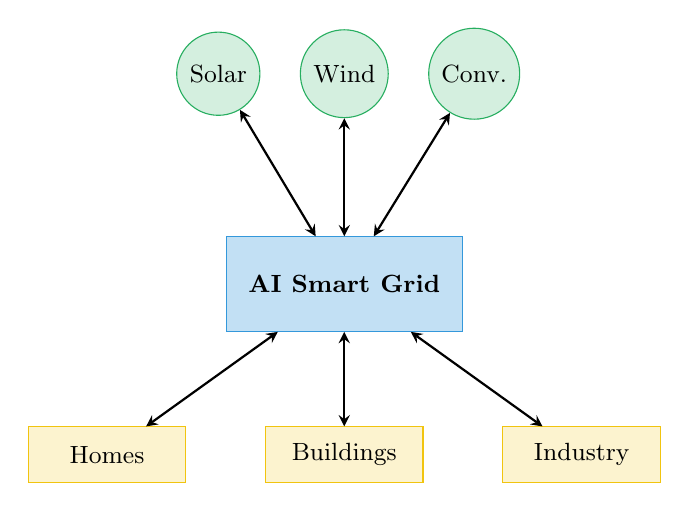
\begin{tikzpicture}[
    node distance=1cm,
    source/.style={circle, draw=greenpower, fill=greenpower!20, minimum size=1cm, font=\small},
    grid/.style={rectangle, draw=gridblue, fill=gridblue!30, minimum width=3cm, minimum height=1.2cm, font=\small\bfseries},
    consumer/.style={rectangle, draw=energyyellow, fill=energyyellow!20, minimum width=2cm, minimum height=0.7cm, font=\small},
    arrow/.style={<->, >=stealth, thick}
]
\node[source] (solar) {Solar};
\node[source, right=0.5cm of solar] (wind) {Wind};
\node[source, right=0.5cm of wind] (conv) {Conv.};

\node[grid, below=1.5cm of wind] (grid) {AI Smart Grid};

\node[consumer, below left=1.2cm and 0.5cm of grid] (home) {Homes};
\node[consumer, below=1.2cm of grid] (building) {Buildings};
\node[consumer, below right=1.2cm and 0.5cm of grid] (industry) {Industry};

\draw[arrow] (solar) -- (grid);
\draw[arrow] (wind) -- (grid);
\draw[arrow] (conv) -- (grid);
\draw[arrow] (grid) -- (home);
\draw[arrow] (grid) -- (building);
\draw[arrow] (grid) -- (industry);
\end{tikzpicture}
\caption{AI-IoT Smart Energy System}
\end{figure}

%==============================================================================
\section{AI-IoT Energy Management Framework}
%==============================================================================

\subsection{Framework Components}

\begin{tcolorbox}[colback=gridblue!10, colframe=gridblue, title=Energy Management Framework]
\begin{itemize}
    \item \textbf{Sensing Layer}: Smart meters, sensors, PMUs
    \item \textbf{Communication Layer}: IoT protocols, networks
    \item \textbf{Data Layer}: Storage, processing, analytics
    \item \textbf{AI Layer}: Prediction, optimization, control
    \item \textbf{Application Layer}: Interfaces, automation
\end{itemize}
\end{tcolorbox}

\subsection{Key Capabilities}

\begin{table}[H]
\centering
\caption{AI Energy Management Capabilities}
\begin{tabular}{lcc}
\toprule
\textbf{Capability} & \textbf{Improvement} & \textbf{Technique} \\
\midrule
Demand Prediction & 15\% MAPE & LSTM, Transformer \\
Load Balancing & 25\% stability & Reinforcement Learning \\
Fault Detection & 95\% accuracy & CNN, Autoencoder \\
Energy Optimization & 20\% savings & Optimization AI \\
\bottomrule
\end{tabular}
\end{table}

%==============================================================================
\section{Smart City Energy Systems}
%==============================================================================

\subsection{Intelligent City Energy}

IoT-enabled urban energy management:
\begin{itemize}
    \item District-level energy monitoring
    \item Smart street lighting control
    \item Electric vehicle charging optimization
    \item Building energy benchmarking
    \item Peak demand management
\end{itemize}

\subsection{Results}

\begin{itemize}
    \item 30-50\% reduction in street lighting energy
    \item 15-25\% building energy savings
    \item Improved grid reliability
    \item Reduced peak demand by 10-20\%
\end{itemize}

%==============================================================================
\section{Generative AI for Low-Carbon AIoT}
%==============================================================================

\subsection{Sustainable AI Infrastructure}

Balancing AI capabilities with carbon footprint:
\begin{itemize}
    \item Energy-efficient model architectures
    \item Carbon-aware computing scheduling
    \item Renewable energy for data centers
    \item LLM optimization for IoT deployment
\end{itemize}

\subsection{Applications}

\begin{itemize}
    \item Natural language energy system queries
    \item Automated energy report generation
    \item Conversational building management
    \item AI-generated efficiency recommendations
\end{itemize}

%==============================================================================
\section{Renewable Energy Integration}
%==============================================================================

\subsection{Forecasting Challenges}

\begin{itemize}
    \item Solar irradiance variability
    \item Wind speed uncertainty
    \item Weather dependency
    \item Grid stability with intermittent sources
\end{itemize}

\subsection{ML Solutions}

\begin{table}[H]
\centering
\caption{Renewable Energy Forecasting}
\begin{tabular}{lcc}
\toprule
\textbf{Source} & \textbf{Model} & \textbf{Accuracy} \\
\midrule
Solar PV & CNN-LSTM & 92\% \\
Wind & Transformer & 88\% \\
Hydro & Random Forest & 95\% \\
Combined & Ensemble & 90\% \\
\bottomrule
\end{tabular}
\end{table}

%==============================================================================
\section{Building Energy Management}
%==============================================================================

\subsection{Smart Building Systems}

IoT-AI integration for buildings:
\begin{itemize}
    \item HVAC optimization through occupancy sensing
    \item Lighting control with daylight harvesting
    \item Plug load management
    \item Predictive maintenance for equipment
\end{itemize}

\subsection{Energy Savings}

\begin{tcolorbox}[colback=greenpower!10, colframe=greenpower, title=Building Energy Results]
\begin{itemize}
    \item HVAC: 20-40\% reduction
    \item Lighting: 30-50\% reduction
    \item Overall: 15-30\% building savings
    \item ROI: 2-4 years typical payback
\end{itemize}
\end{tcolorbox}

%==============================================================================
\section{Challenges and Solutions}
%==============================================================================

\subsection{Data Integration}

\begin{itemize}
    \item Heterogeneous energy data formats
    \item Legacy system connectivity
    \item Solutions: Standardization, middleware, APIs
\end{itemize}

\subsection{Real-Time Control}

\begin{itemize}
    \item Latency requirements for grid stability
    \item Computational demands of optimization
    \item Solutions: Edge computing, efficient algorithms
\end{itemize}

%==============================================================================
\section{Future Directions}
%==============================================================================

\begin{enumerate}
    \item \textbf{Autonomous Energy Systems}: Self-managing grids
    \item \textbf{P2P Energy Trading}: Blockchain-enabled markets
    \item \textbf{Vehicle-to-Grid}: EV as distributed storage
    \item \textbf{Hydrogen Integration}: AI for hydrogen systems
    \item \textbf{Carbon-Neutral AI}: Sustainable ML infrastructure
\end{enumerate}

%==============================================================================
\section{Conclusion}
%==============================================================================

AI-driven IoT systems are essential for modern energy management, enabling significant efficiency gains and renewable integration. Smart grid systems improve stability by 25\%, while building management reduces consumption by 15-30\%. Generative AI enables natural language interaction and automated optimization. Key challenges in data integration and real-time control are being addressed through standardization and edge computing. Future developments in autonomous systems and peer-to-peer trading will further transform energy management toward sustainability.

%==============================================================================
% References
%==============================================================================
\bibliographystyle{plainnat}
\begin{thebibliography}{10}

\bibitem{ai_iot_energy2025}
Wang, C. \& Liu, Y. (2025).
\newblock Introducing AI-Driven IoT Energy Management Framework.
\newblock {\em arXiv preprint arXiv:2512.00321}.

\bibitem{smart_city_energy2023}
Wang, Y. \& Li, C. (2023).
\newblock Intelligent Energy Management in Smart Cities: Leveraging IoT.
\newblock {\em arXiv preprint arXiv:2306.05567}.

\bibitem{genai_low_carbon2024}
Li, M. \& Chen, H. (2024).
\newblock Generative AI for Low-Carbon Artificial Intelligence of Things with Large Language Models.
\newblock {\em arXiv preprint arXiv:2404.18077}.

\end{thebibliography}

\end{document}
